\documentclass{article}
\usepackage[utf8]{inputenc}
\usepackage[margin=2.6cm]{geometry}
\usepackage{float}
\usepackage{rotating}
\usepackage{graphicx}
\usepackage{caption}
\usepackage{subcaption}
\usepackage[round]{natbib}
\usepackage{setspace}
\usepackage{longtable}
\usepackage{lscape}
\onehalfspacing
\usepackage{tikz}
\usetikzlibrary{arrows,automata,positioning,shapes}
\usepackage{adjustbox}
\usepackage{amsmath}
\usepackage{tabularx}
\usepackage{multirow}
\usepackage{algorithm}
\usepackage{algpseudocode} 

\title{The role of resource dynamics in the distribution of life cycles within a female human population.
\\
Registered Report}
\author{Pablo J. Varas Enriquez, Daniel Redhead, Monique Borgerhoff Mulder,
\\
Heidi Colleran, Dieter Lukas}
\date{\today}

\begin{document}

\maketitle

\tableofcontents

\begin{abstract}
    The female human life cycle is characterised by a long lifespan with a typically short reproductive career, which is between long juvenile and post-reproductive stages. There is a high diversity on how different life history traits that characterise such life cycle distribute within a population. This variability may reflect how individuals face different trade-offs to allocate resources between survival and reproduction. Formal theoretical models have proposed that the surplus resources produced during adulthood, and inter-generational resource transfers towards juveniles, have driven the evolution of the female human life cycle. However, these models focus on the conditions under which the average life cycle emerges, and remains unclear how production and resource transfers (i.e. resource dynamics) shape the variability of life history traits within a human population as well. Here, we develop a theoretical framework to describe how different resource dynamics influence the average and variability of life cycles within a female human population. First, we focus on how resource production shape the distribution of life history traits within a female human population. Then, we analyse how the interplay between production and resource transfers influences the distribution of life cycles. And finally, we aim to understand how this relationship might vary when individuals vary in the amount of resources they can acquire from the environment. We build a computational model to answer these three research questions, using a stage-structured sub-model that dictate stochasticity in resource production, and a stage-structured stochastic block model to define the network structure of resource transfers. Regarding the life history traits, the allocation of resources towards them is deterministic and is based on surpassing the amount of resources set as thresholds for survival and reproduction. We expect that the individual differences in resource dynamics, and how they influence the allocation of resources towards survival and reproduction, will help to understand the mechanisms behind the diversity of life cycles observed within human populations. Furthermore, exploring the relationship of resource dynamics with the female human life cycle may reveal potential buffering effects resulting from resource transfers and/or compensatory mechanisms that could arise from resource production, thus shedding light on the overall role of resources in shaping the human life cycle.
\end{abstract}

\section{Introduction}

There are many paths an individual can follow through its life cycle, which is the basis of the diversity seen across the tree of life. The diversity of mortality schedules can lead to lifespans that vary from days to thousands of years (e.g. hairyback vs patagonian cypress \citep{balsamo1988life,lara19933620}) and reproductive outputs can go from a couple to thousands of offspring (e.g. eastern hemlock vs rain moth \citep{tindale1932revision,van2017lifetime}. Within the tree of life, the female human life cycle is characterised by a long lifespan and a short reproductive career, framed within long juvenile and post-reproductive stages \citep{kaplan2000theory}. Within these boundaries, the life cycle of female humans also varies in terms of mortality and fertility. Populations can differ in their average life expectancy by a factor of 2 and their average reproductive output by a factor of 5 (e.g. foraging populations \citep{migliano2007life} versus post-demographic transition populations \citep{de2017maximum}). The diversity of life cycles observed among female human populations is fuelled by the differences in longevity and fertility between individuals within a population. For example, there is record of childlessness up to 40\% among populations with high fertility rates of sub-Saharan Africa, and more specifically there is evidence that 28\% of Efe women being childless \citep{bailey1995sexuality,belsey1976epidemiology}. However, it is not clear if the diversity of life cycles within female human populations is explained by the same processes that explain the differences seen among species. 

The differences in life cycles among species have usually been related to the trade-offs in which an individual allocates the limited resources available in its environment towards life history traits such as survival or reproduction \citep{stearns2000life}. The fast-slow continuum is a key life history framework to explain differences at the species level, where some species show a ``fast" strategy by having a short lifespan but a high reproductive output whereas those with a ``slow" strategy live longer but reproduce less \citep{stearns1983influence}. However, further analyses have shown that life history strategies among species have more than one dimension, showing that reproductive strategies \citep{salguero2016fast}, the distribution of mortality risk \citep{healy2019animal}, and individual stochasticity \citep{varas2022individual} play major roles in the explanation behind the diversity of life cycles across the tree of life. Hence, the space under which different life cycles emerge, and evolve, should be understood considering the environmental constraints experienced by individuals, and how individuals resolve these constraints through the allocation of resources towards growth, survival, or reproduction \citep{white2022metabolic}.

The individual differences in longevity within human populations have been associated with resource availability (i.e. more resources equals longer lifespans) \citep{kaplan2003embodied}, whereas the relationship of resources with fertility outcomes is more complex \citep{mulder1998demographic,sear2016understanding}. Resource transfers have been proposed as a key component to understand the different life cycles among female humans, due to the social nature of our species. Here, the presence of different members of the population have been associated with differences in the longevity and reproductive output of female individuals, as can be found in the literature related to communal breeding, sibling competition, female conflict, among others \citep{ivey2000cooperative,nitsch2013elder,mace2012female,sear2011much}. However, research in the area usually focus on specific life history traits of the life cycle (e.g. longevity, number of descendants) rather than addressing them together, and/or specific ways in which resources are available for female individuals (e.g. amount of food, presence of the grandmother). Therefore, the understanding of the mechanisms linking the diversity of life cycles within a female human population with resource availability remains limited.

Evolutionary models that focus on the differences in longevity and reproduction among individuals have been developed in terms of early life conditions and the balance between resource acquisition and allocation. Here, the silver spoon model proposes that individuals who experience good conditions early in life will perform better in every environment as adults \citep{pigeon2019silver,lummaa2002early}. The adaptive developmental plasticity model proposes that individuals who develop a phenotype in response to the inputs they receive early in life should be the ones with a higher fitness than their counterparts, whereas those who do not experience the early-life inputs and/or do not develop the phenotype show a higher fitness than those who develop the phenotype without early-life inputs \citep{bateson2004developmental,nettle2015adaptive}. The environmental saturation model suggests that the environmental and/or physiological constraints impose fitness limits, where individual differences would mostly be seen in environments with intermediate conditions, while in good and poor environments fitness would be more homogeneous among individuals \citep{engqvist2016adaptive}. The work relating resource acquisition and allocation is mainly based on the work of \cite{van1986acquisition}. Here, they show that with high variability of resource acquisition comes a low variability of resource allocation towards reproduction, which makes that individuals who live longer also have the highest reproductive output within a population (i.e. phenotypic masking). Recent reviews from the pace-of-life syndrome framework on their model show that resource acquisition plays an equal, or bigger, role than resource allocation to understand the differences in survival and reproduction among individuals, phenotypes, and within individuals \citep{laskowski2021integrating,haave2022differences}. However, neither of the approaches consider the social basis that comes with resource transfers among individuals, which diversify the ways in which resources or inputs are acquired and distributed.    

Models that address the limitations of how the life cycles of women in a population are shaped by resource acquisition focus on the conditions that differentiate the female human life cycle from other species. The ``embodied capital model" suggests that the surplus of resource production during adulthood allows the evolution of the female human life cycle \citep{kaplan2000theory}. This model proposes that the difference between resource production and consumption allows high parental investment, translated in short interbirth intervals and long post-reproductive periods for the parents and long juvenile periods for their offspring. The ``pooled energy model" deepens in this framework by suggesting that alloparenting from individuals of different generations would allow to decrease the load of parental investment \citep{kramer2010pooled}. The ``inter-generational resource transfer model" poses that inter-generational transfers would play a major role in the mortality and fertility schedules of human populations. As developed by \cite{lee2003rethinking}, this model suggests that age-specific mortality is proportional to the remaining reproductive value and resource transfers made at later ages, predicting the early-life and later-life mortality patterns characteristics of the female human life cycle. Additionally, Chu and Lee further develop the ``inter-generational resource transfer model", showing that transfers co-evolve with low mortality, since adults are more efficient to produce energy, which is transferred to juveniles, who are more efficient to turn that energy into body size, allowing lower mortality \citep{chu2006co}. While these models show that the female human life cycles co-evolved with the interplay of resource acquisition and transfers, they do not address how different resource dynamics can shape the variability of life cycles within a population.

Our aim is to develop a theoretical framework to understand how the environmental constraints and the individual resource dynamics (i.e. resource production, transfers, and storage) influence the variability of life cycles within a female human population (see a summary in Table \ref{tab:1}). The model will explore the influence of habitat quality by setting different values for the amount of resources that can be acquired from the environment, while the influence of resource dynamics will be characterised by different stochastic probabilities of production and transfers. The framework will be developed with an agent-based model, because of its capacity to address complex phenomena from individual and population levels, as well as address stochasticity among individuals by allowing agents to behave differently despite being all under the same rules \citep{judson1994rise,wilensky2015introduction}. In the following section, we describe the model using an ODD (Overview, Design concepts, Details) protocol, as an standardised way to clarify the scope, assumptions, and parameters used to answer our questions \citep{grimm2006standard,grimm2020odd}. The development of this model will allow to understand the conditions and mechanisms that allow higher variability of life history traits despite being under strong selection pressures. Furthermore, the results will help to further understand the demographic diversity observed among human populations, as well as offer a tool to further test the complexity of the environmental and social components that link resource availability with the development of life cycles.

\section{Model description}

\subsection{Purpose and patterns}

The purpose of the model is to understand how different resource dynamics influence the distribution of female life cycles within a population. The mechanism expected to influence the life cycle at an individual level is the interplay of resource production and transfer which allows individuals to allocate resources to survival, life stage transitions, and reproductive timing and output. The variability of female human life cycles at the population level would be explained by the distribution of different life cycles that arise from individual differences. The expected patterns can be described based on the resource dynamics that individuals experience. First, an increase in the individual probabilities of resource production would increase the average life cycle in the population whereas the variability would show an inverted U-shaped pattern. These patterns would be expected because, for the average, if more individuals produce resources then more are allowed to live longer and reproduce more, whereas for the variability, individuals would experience more homogeneous resource dynamics on the extreme individual probabilities (e.g. everyone is poor or rich) allowing less diversity in resource allocation towards survival and reproduction. Second, the patterns described above would be more extreme if the amount of resources than an individual can produce increases. Hence, the average life cycle would increase more and the variability would show a shape with higher kurtosis. Finally, the inclusion of resource transfers would have a buffering effect, where the increase of the average life cycle and the inverted U-shaped pattern in variability would be more smooth compared to the patterns described before. The buffering effect would be explained because of the redistribution of resources within a population would allow indidivuals to avoid extreme life cycles (e.g. having no descendants or shorter lifespans) (see Table \ref{tab:1} and \ref{tab:2} for a summary).
\\\\
The life cycle of an individual is described by her longevity, lifetime reproductive output, and the timing of life cycle stage transition. Longevity is the total number of years alive, whereas her lifetime reproductive output is the total number of descendants throughout her life. The timing of life cycle stage transition refers to the age at which an individual transitions through four discrete stages (i.e. juvenile, adult, reproductive-career, post-reproductive). Each transition represents a specific event in the life cycle of an individual: age at menarche, age at first reproduction, and age at menopause.
\\\\
The resource dynamics will be characterised by the amount of resources available, produced, transferred, and stored throughout the life cycle. Resources available is the total amount of resources that an individual has before allocating resources towards survival, reproduction, and life cycle transition. Production is the amount of resources that an individual can acquire from her habitat by herself. Resource transfer is understood as the sharing dynamics where an individual gives and receives resources towards or from other individuals in the population. Storage of resources is described as the amount of resources that pass from one iteration to the next one. Finally, there will be different scenarios based on combinations of probabilities of resource production and transfers (i.e. high and low) as well as habitat quality (i.e. high and low) (see Table \ref{tab:2} for a summary).

Resource transfer is understood as the sharing dynamics where an individual gives and receives resources towards or from other individuals in the population. The number of transfers is randomly determined by the surplus of resources available (i.e. produced plus stored). The amount of resources transferred is determined by the amount of resources available and the number of transfers. To whom resources are transferred is based on probabilities that would determine the likelihood of giving, or receiving, resources to, or from, individuals in specific life cycle stages over others depending on the stage of the individual. 
\\\\
The influence of resource dynamics into the life cycle will be understood by the differences between individuals within a population in their life history traits (i.e. longevity, lifetime reproductive output, age at menarche, age at first reproduction, and age at menopause). A graphical representation of the ways in which resource dynamics influence the life cycle can be seen in Fig. \ref{fig:1}.

\subsection{Entities, state variables, and scale}

\subsubsection{Entities}

An individual represent females in a single-sex population. A single-sex population is used because the model is focused on the female human life cycle, under the assumption that it evolves independently from the male counterpart. Individuals that are born until they reach age of menarche are considered juveniles. Adults are individuals that have reached menarche until they have their first descendant or reach menopause. Adults transition to a reproductive-career stage once they have their first reproduction, and remain in this stage until they reach menopause. From menopause onward individuals are considered post-reproductive. The population is run for a single generation, without inheritance or long-term adjustments, since we only record the reactions of individuals to the given conditions.

\subsubsection{State variables}

Every individual in the simulation is characterised by state variables that are either calculated new in each iteration or modified from one iteration to the next. First, we describe the variables related to resource dynamics, followed by the ones about life history dynamics.

\paragraph{Resource dynamics}

\subparagraph{Production:}

Is the amount of resources produced by an individual. The amount is calculated by randomly sampling a value from a Binomial distribution. The distribution is defined as:

\begin{equation}
    RP_{i,t} \sim \text{Binomial}(maxRP_S,P_S)
\end{equation}

Where $RP_{i,t}$ is the amount of resources produced by individual $i$ at time $t$, $maxRP_S$ the maximum amount of resources an individual can produce at stage $S$, and $P_{S}$ the probability of resource production at stage $S$.

\subparagraph{Maternal investment:}

Is the amount of resources an individual transfers to her descendants. An individual would transfer resources to her descendants that do not have enough resources to cover the costs of survival. If she does not have enough resources to cover the need of her descendant, she will transfer resources to the next one that needs resources or not transfer resources if there are no more descendants. The amount is based on the surplus of resources that an individual has, and the need that her descendant(s) have. Hence, maternal investment would be defined as:

\begin{equation}
    MI_{i,t}=\begin{cases}
    MS_{i,t}- DN_{j,i}& \text{, } MS_{i,t} > S_c \wedge MS_{i,t} \geq DN_{j,i}\\
    0 & \text{, } MS_{i,t} < DN_{j,i}
\end{cases}
\end{equation}

Where $MI_{i,t}$ is the amount of maternal investment of individual $i$ at time $t$, $MS_{i,t}$ is the maternal surplus of individual $i$ at time $t$, $DN_{j,i}$ is the descendant need of descendant $j$ from individual $i$, $RA_{i,t}$ is the amount of resources available of individual $i$ at time $t$, and $S_c$ is the survival cost.

The maternal surplus is defined as:

\begin{equation}
    MS_{i,t}=RA_{i,t}-S_c
\end{equation}

Where $MS_{i,t}$ is the maternal surplus of individual $i$ at time $t$, $RA_{i,t}$ is the amount of resources available of individual $i$ at time $t$, and $S_c$ is the survival cost.

The amount of resources available for an individual $i$ at time $t$ ($RA_{i,t}$) after maternal investment would be defined as follow:

\begin{equation}
    RA_{i,t}=RA_{i,t}-MI_{i,t}
\end{equation}

Whereas, the amount of resources available for a descendant $j$ at time $t$ ($RA_{j,t}$) after manternal investment would be defined as:

\begin{equation}
    RA_{j,t}=\begin{cases}
    S_c& \text{, } MS_{i,t} \geq DN_{j,i}\\
    RA_{j,t} & \text{, } MS_{i,t} < DN_{j,i}
\end{cases}
\end{equation}

\subparagraph{Resource transfers:}

Is the amount of resources transferred to other individuals within the population. Every tie an individual has in the social network represents the transfer of one resource unit to another individual. Therefore, an individual will transfer more resources if she forms more ties within the social network. The number of ties an individual forms within the network is randomly assigned using a stochastic block model. The maximum number of ties an individual can form is defined by the surplus of resources that she has available in the iteration:

\begin{equation}
    Maxdeg_{i,t}=SR_{i,t-1}+RP_{i,t}-MI_{i,t}-S_c
\end{equation}

Where $Maxdeg_{i,t}$ is the maximum outdegree of individual $i$ at time $t$, $SR_{i,t-1}$ is the stored resources from the previous iteration, $RP_{i,t}$ and $MI_{i,t}$ are the amount of resources produced and maternal investment of individual $i$ at time $t$, respectively, and $S_c$ is the survival cost.

The block matrix with the stage-specific probabilities of forming ties within and between life cycle stages is defined in the ``auxiliary variables" section.

The amount of resources that an individual transfers to another one is the out degree of the individual in the social network. The amount of resources an individual receives is the in degree.

\subparagraph{Resources available:}

Is the amount of resources that an individual has after the resource dynamics of production, maternal investment, and resource transfers to cover the costs of survival, reproduction, and life cycle stage transition. The amount is calculated as:

\begin{equation}
    RA_{i,t}=RS_{i,t-1}+RP_{i,t}-MI_{i,t}-RT_{i,t}+RR_{i,t}        
\end{equation}
        where $RA_{i,t}$ is the amount of resources available for individual $i$ at time $t$, $RS_{i,t-1}$ the stored resources from the previous iteration ($t-1$), $RP_{i,t}$ the amount of resources produced, $MI_{i,t}$ the maternal investment, $RT_{i,t}$ and $RR_{i,t}$ the resources transferred and received at time $t$.

\subparagraph{Stored resources:}      

Is the amount of resources the individual stores for later in time (i.e. next iteration). The amount of resources stored depends on the surplus resources after the resource and life-history dynamics experienced by an individual in the iteration. Stored resources is defined as:

\begin{equation}
    SR_{i,t}=RA_{i,t} - R_c - T_c - S_c 
\end{equation}
    Where $SR_{i,t}$ is the amount of resources stored by individual $i$ at time $t$, $RA_{i,t}$ is the amount of resources available for individual $i$ at time $t$, $R_c$ is the reproductive cost, $T_c$ is the costs of life cycle stage transition, and $S_c$ is the survival cost.
    
\paragraph{Life history dynamics}

\subparagraph{Reproduction:}

Whether an individual has a descendant (1) or not (0) in the iteration depends if she has enough resources available to cover the reproductive costs. Reproduction is defined as:

\begin{equation}
    R_i=\begin{cases}
    1,& RA_{i,t} \geq R_c\\
    0,& RA_{i,t} < R_c
\end{cases}
\end{equation}
        Where $R_i$ is the reproductive output of individual $i$, $RA_{i,t}$ is the amount of resources available for individual $i$ at time $t$. $R_c$ is the reproductive cost.

\subparagraph{Transition:}
       
Whether an individual transitions to the next life cycle stage, depends if she has enough resources available to allocate towards the key event of transition.
\begin{equation}
    T_i=\begin{cases}
    T_{J \to A},& RA_{i,t} \geq S_c+R_c \wedge AGE_{i,t} \geq 10 \vee AGE_{i,t} \geq 18\\
   T_{A \to RC},& RA_{i,t} \geq R_c\\
   T_{A \to PR},& AGE_{i,t} \geq 60\\
   T_{RC \to PR},& RA_{i,t} \leq R_c \wedge TLR_{i,t} \geq 10 \wedge AGE_{i,t} \geq 40 \vee AGE_{i,t} \geq 60\\
\end{cases}
\end{equation}

Where $T_i$ is the transition output of individual $i$, $RA_{i,t}$ is the amount of resources available, $S_c$ is the survival cost, $R_c$ is the reproductive cost, $AGE_{i,t}$ is age, and $TLR_{i,t}$ is the time since last reproduction of individual $i$ at time $t$, respectively. $T_{J \to A}$, $T_{A \to RC}$, $T_{A \to PR}$, $T_{RC \to PR}$ are the transitions from one life cycle stage to the next one.
        
The transitions are defined as follow:
        \begin{itemize}
            \item Age at sexual maturity ($T_{J \to A}$): A juvenile female individual reaches menarche once she has enough resources to cover the costs of survival and reproduction, and is at least 10 years old. If the individual reaches 18 years old she is forced to reach sexual maturity, regardless of the amount of resources available. The minimum and maximum ages of sexual maturity are based on \cite{morabia1998international} and \cite{kramer2010teen}.
            \item Age at first reproduction ($T_{A \to RC}$): An individual in the adult stage transitions to a reproductive career stage as she has her first descendant. The first descendant would happen when the individual has enough resources to cover the survival and reproductive costs. Afterwards, she gets discounted the reproductive cost from her resources available.
            \item Age at menopause ($T_{RC \to PR}$, $T_{A \to PR}$ and $T_{RC \to PR}$): A female individual reaches menopause once she has enough resources to cover the survival costs but has not covered the costs for reproduction in the last 10 iterations, based on \cite{towner2016women}. She will be forced to transition if she is 60 years old based on \cite{morabia1998international} and \cite{thomas2001international}.
        \end{itemize}

\subparagraph{Survival:} 

Whether the individual survives (1) or not (0) in the iteration, which depends if the individual has enough to cover the survival cost. The survival is defined as:

\begin{equation}
    S_i=\begin{cases}
    1,& RA_{i,t} \geq S_c\\
    0,& RA_{i,t} < S_c
\end{cases}
\end{equation}
        Where $S_i$ is the survival output of individual $i$, $RA_{i,t}$ is the amount of resourced available by individual $i$ at time $t$, and $S_c$ is the survival cost.

\subparagraph{Age:} 

Is the amount of iterations the individual goes through from its birth until it dies ($AGE_{i,t}$). Age increases by one after each iteration, reflecting one year.
        
\subparagraph{Lifetime reproductive output:}

Is the total number of descendants produced ($LRO$). The reproductive output increases by one if the individual reproduces in the iteration.

\subparagraph{Stage:}

Is the life cycle stage in which the individual is at the moment ($S_i$). The stage changes if the individual fulfils  the requirements to move to the next life cycle stage in the iteration ($T_i$). There are four stages (juvenile, adult, reproductive-career, post-reproductive), each with its own stage-specific resource dynamics.
 
\subsubsection{Auxiliary variables}

The individual dynamics related to the state variables are constrained by the following auxiliary variables. These variables are stage-specific, set at the initialisation and apply to all individuals. The auxiliary variables related to resource dynamics are described first, followed by the ones regarding life history dynamics.

\paragraph{Resource dynamics}

\subparagraph{Production probability:}

Probability of producing resources ($P_S$) that is used in the state variable ``Production".

\subparagraph{Maximum resource production:}

Is the maximum amount of resources an individual can produce in the iteration ($maxRP_S$).

\subparagraph{Block matrix:}

Is the directed relational matrix with the probabilities of forming ties within and between life cycle stages (i.e. blocks). The block matrix is defined as:

$
B=
\begin{pmatrix}
      J \to J & J \to A & J \to RC & J \to PR \\
      A \to J & A \to A & A \to RC & A \to PR \\
      RC \to J & RC \to A & RC \to RC & RC \to PR \\
      PR \to J & PR \to A & PR \to RC & PR \to PR
\end{pmatrix}
$  

Where every value in the matrix ($S_i \to S_j$) is the probability that an individual $i$ transfers resources to individual $j$, depending on the life cycle stage of each of them ($S$).
    
\paragraph{Life history dynamics}

\subparagraph{Reproductive cost:}

Is the amount of resources necessary to produce a descendant ($R_c$).

\subparagraph{Number of descendants per reproduction:}

Is the number of descendants that an individual can produce per reproductive event.

\subparagraph{Survival cost:}

Is the amount of resources needed to survive until the next iteration ($S_c$).

\subsubsection{Scale}

Each iteration in the model represents one year. The probability  of producing is Bernoulli, with the values of happening ($1$) or not ($0$). The times that resources are received or gave away can be a minimum of zero (i.e. no receiving/giving) and a maximum based on the surplus of resources available and the dynamics set in the stochastic block model. The amount of resources and probability that an individual produces, receives, and gives are stage-specific. Survival and reproductive effort are evaluated after the resource dynamics, followed by the evaluation for stage transition. Finally, the amount or resources available are stored and passed from one year to the next.

\subsection{Process overview and scheduling}

Every dynamic described in the following process is stage-specific. In the juvenile stage, individuals go through the produce, sharing, and survive models each year until they reach sexual maturity, transitioning to the adult stage. In the adult stage, individuals go through produce, sharing, and survive models until they have their first descendant or reach menopause. If an adult transitions to a reproductive-career stage, she goes through produce, maternal investment, and sharing models followed by reproduction and survive models until she reaches menopause. Once in a post-reproductive stage, the individual goes through the produce, maternal investment, sharing, and survive models of the stage. In each year, the individual increase her age and updates the amount of resources she stores. During each transition, the individual updates her stage variable and also transitions with the resources she has stored from the earlier stage.
\\\\
The scheduling of the process starts with the production model, followed by the maternal investment model if an individual is in the reproductive-career stage. The sharing model happens afterwards, followed by the reproduction, transition models. The decrease of resource available comes first from the amount of resources produced by the individual in that iteration, and the ones stored afterwards. The resource allocation towards the life history traits that characterise the life cycle happens after the resource dynamics to evaluate the influence of resource availability in the life cycle. The schedule ends with the survive model to evaluate if the individual moves to the next iteration or not.

\subsection{Design concepts}

\subsubsection{Basic principles}

The model aims to understand how the variability of life cycles within a population change based on the influence of different resource dynamics and habitat qualities. Models so far have focused on the conditions under which the female human life cycle evolved (e.g. embodied capital model \citep{kaplan1996theory} or resource transfer model \citep{chu2006co}), while the model here differs from them by focusing on the mechanisms behind the variability of life cycles. Additionally, the model is more explicit in the resource dynamics than previous models \citep{price2020fitness,kaplan1996theory,chu2006co,lee2003rethinking,kramer2010pooled, van1986acquisition}. First, resource transfers are defined more general, and not bounded to specific relationships among individuals (e.g. parent-offspring transfers as in \cite{kaplan1996theory} or downward adult-juvenile transfers as in \cite{chu2006co}). Second, resource transfers are modelled independently instead as a byproduct of other resource dynamics (e.g. giving as a positive outcome from resource production and consumption, and receiving as a negative one, as in \cite{lee2003rethinking,chu2006co}). Finally, the model is driven by mechanistic processes since the individual survives, reproduce, and transition through the life cycle depending on the amount of resources she has. Therefore, individuals have a deterministic behaviour in terms of the allocation of resources towards survival and reproduction, whereas resource acquisition and sharing is a stochastic one.

\subsubsection{Emergence}

The life cycle of an individual emerges from its behaviour in terms of resource dynamics. The life cycle is represented by the timing of key events of the life course (i.e. life stage transition, reproductive output and timing, and longevity) constrained by the stage-specific resource dynamics. Population dynamics emerge from the behaviour of the individuals. The population dynamics are represented as the age distributions of the life cycle transitions, reproductive output and timing, and longevity and surviving individuals. The aim is to understand how the resource dynamics (i.e. production, transfer, storage) experienced by individuals within a population cause changes in the variability of different components of the female human life cycle (i.e. longevity, age at menarche, age at first reproduction, number of descendants, average interbirth intervals, age at last reproduction, age at menopause).

\subsubsection{Adaptation}

The primary adaptive behaviour of an individual is to allocate resources towards survival and/or reproduction. The adaptive behaviour shapes the life cycle of an individual because it determines the longevity, the reproductive output and timing, and the transition from one life cycle stage to another. Whether an individual survives, reproduces, or transitions in one iteration depends on having enough resources to satisfy the thresholds set for survival, reproduction, and transition set at initialisation. The amount of resources available for survival and reproduction is determined by maternal investment and stochastic resource dynamics. Maternal investment follows a need-based behaviour, where an individual allocates resources to those descendants that do not have enough resources to cover the costs of survival. The stochastic resource dynamics are determined by stage-specific probabilities of producing resources, based on a Bernoulli probability distribution, as well as for giving and receiving resources, based on the stochastic block model. 

\subsubsection{Learning}

There is no learning process for the individuals in the population because the model focuses on the environmental constraints and resource dynamics under which the female human life cycle varies.

\subsubsection{Prediction}

The adaptive behaviour of an individual is based on the implicit prediction that moving to the next life stage, reproducing, and/or surviving when having the necessary amount of resources is likely to result in individuals having a life cycle that has the longest lifespan, and the highest reproductive output. This life cycle would be possible by expanding their time in the reproductive career stage (i.e. reaching sexual maturity and starting reproduction earlier, while stopping reproduction and reaching menopause later). On the other extreme, individuals are likely to have life cycle with short lifespan and low reproductive output when they do not have enough resources to allocate. This life cycle would have long time before reaching sexual maturity and starting reproduction, while it would stop reproduction and reach menopause earlier. Variations of these predictions can be expected by differences in the amount of resources that an individual experiences through its life cycle, being more sensitive to changes in resource production, whereas transfers and storing dynamics should have a buffering effect.
\\\\
At the population level, it should be expected that variability of life cycles is lower in populations where individuals are more homogeneous in the resource dynamics they experience, while the variability increases as individuals are more likely to experience different amounts of resources and outcomes from their decision processes, especially by differences in resource production.

\subsubsection{Sensing}

Individuals are assumed to know their stage, and their current resources produced and stored in order to determine the resource transfer dynamics. Furthermore, they are assumed to know the amount of resources available after the transfers dynamics to allocate them into reproduction, life cycle stage transition, and/or survival. Finally, they are assumed to know the amount of resources left at the end of the iteration to store them and carry them to the next iteration.


\subsubsection{Interaction}

Individuals randomly interact with one another during the resource transfers. Here, the number of interactions are determined by the number of times an individuals randomly forms within the sharing network. The sharing network is based on a stochastic block model with a maximum upper bound depending on the resource surplus of each individual. The model assigns stage-specific probabilities of forming ties within and between life cycle stages.

\subsubsection{Stochasticity}

Resource dynamics are stochastic in the model since they are based on probability distributions. Individuals produce resources within an iteration based on randomly sampling a value from a Bernoulli distribution with an upper bound based on the stage-specific maximum resource production. The sharing dynamics are also stochastic because the number of times and with whom resources are transferred are also based on probability distributions specified in the stochastic block model. Individuals survive, reproduce, and transition from one life stage to another by reaching a certain amount of resources. Therefore, the resource dynamics of an individual are stochastic, whereas resource allocation is determined by the amount of resources available.

\subsubsection{Collectives}

Not apply

\subsubsection{Observation}

The purpose of the model is to identify which scenarios of resource dynamics and habitat quality vary the timing of life stage transitions, longevity, and reproductive timing and output of individuals. Therefore, the different resource dynamics (i.e. production, sharing, storing) and the timing and output of the different components of the life cycle are recorded for each individual. At the population level, distributions of each trait of the female human life cycle as well as resource dynamics are produced based on the individual data.

\subsection{Initialisation}

At initialisation, the population will be composed of equal number of individuals per life cycle stage, which will start with resources depending on their life cycle stage. For juveniles, they will start with age zero and no resources since they are newborns in the population. Individuals in the adult and reproductive career stages will start with ages sampled from a normal distribution with average 14 and standard deviation of 1 ($\text{Adult}\sim \text{Normal}(14,1)$), and a normal distribution with average 22 and standard deviation of 1 ($\text{Reproductive career}\sim \text{Normal}(22,1)$), respectively \citep{kramer2010teen,morabia1998international,thomas2001international}, and the amount of resources stored one iteration after reaching the reproductive threshold, that is used to establish the transition of both life cycle stages (i.e. age at menarche and age at first reproduction). Individuals in their post-reproductive stage will start with ages sampled from a normal distribution with average 50 and standard deviation of 2 ($\text{Post-reproductive}\sim \text{Normal}(50,2)$) \citep{morabia1998international,thomas2001international} and the amount of resources stored after reaching the conditions to reach menopause. 
\\\\
The auxiliary variables for each stage are set at initialisation.

\subsection{Input Data}

The model does not use input data to represent time-varying processes.

\subsection{Sub models}

Not apply

\section{Model Analysis}

The model analysis consists on running simulations where the resource dynamics and habitat quality are considered the input parameters while the components of the life cycle are the output. Different combinations of resource dynamics and habitat quality will be used to analyse the influence of each input parameters in the variability of female life cycles, recording them at the individual and population level. Two levels for each resource dynamic (high, low) and two levels of habitat quality (high, low) are considered to define the different scenarios that the model will be tested, together with a baseline scenario with values between the two levels. Regarding the components of the life cycle, the timing of life stage transitions, reproductive output and timing, and longevity will be recorded for each individual. Additionally, distributions will be built from the individual records to estimate the variability of the different components of the life cycle.

\section{Future modifications}

The model will be modified to set the different scenarios of interest to understand how resource dynamics and habitat quality influence the variability of life cycles within a female human population. The probabilities of resource production and transfers will be modified with different combinations of higher and lower values than the baseline model developed here. Additionally, the amount of resources that can be produced will be set with higher values than the ones in the baseline to compare rich and poor environments. See Table \ref{tab:2} for a summary of the different scenarios that will be set, and the expected predictions.

\section{Tables and Figures}

\begin{table}[H]
    \centering
    \caption{Summary of the study design. \emph{Question} is where are the research questions driving the development of the model. \emph{Hypothesis} is where are the predictions answering the research questions. \emph{Analysis plan} is where the tests used to answer the research question are described. \emph{Interpretation} is a description of possible different outcomes, and their interpretation in relation to the hypothesis. \emph{Contested theory} is a description on how the possible outcomes could prove wrong or show incomplete current theories.}
    \begin{adjustbox}{width=\textwidth}
    \begin{tabular}{p{4cm}p{4cm}p{4cm}p{4cm}p{4cm} }
    \hline
    Question & Hypothesis & Analysis plan & Interpretation & Contested Theory \\ 
    \hline
    How does the distribution of life cycles within a female human population change under different probabilities of resource production? & The life cycle average increases as resource production probability is higher. The variability of life cycles decreases as resource production probabilities become more homogeneous, resulting in an inverted U-shaped pattern between life cycle variability and resource production probabilities. This relationship shows the highest variability when production probabilities are moderate. & Three scenarios with different production probabilities: baseline, high, and low. The baseline would be a moderate scenario, the high one would be with double the probability from the baseline, and the low scenario would be with half the probability from the baseline. In each scenario the output would be the average and variability of each life history trait, and of all resources available, produced, and transferred. & Greater resource production probability can enhance the average life cycle of a population by enabling more individuals to obtain resources that support extended lifespan and increased reproduction. In terms of life cycle variability, low and high probabilities of resource production lead to more uniform life cycles due to individuals facing similar conditions of scarcity or abundance. & The results would fill a gap in the understanding on the roles of production in the life cycles of female individuals within human populations, especially to understand how the average and variability of life history traits behave differently in relationship with resource production.\\
    
    How does the distribution of life cycles within a female human population change under different probabilities of resource production and transfers? & As production and transfer probabilities increase, the average life cycle of a population also increases, albeit at a diminishing rate when transfers are included. This is because individuals not only use resources for their own survival and reproduction but also distribute them within the population. Homogeneity in resource production and transfers results in decreased variability in life cycles. A inverted U-shaped pattern is observed when transfer probabilities are low, as resource redistribution buffers extreme life cycles. & Multiple scenarios with different combinations of production and sharing probabilities (i.e. high, baseline, and low). In each scenario the output would be the average and variability of each life history trait, and of all resources available, produced, and transferred. & Resource transfers buffers the effects of resource fluctuations on the average and variability of life cycles within a population. Resource redistribution enables individuals to avoid extreme life cycles. When the probability of resource production is low, increasing resource transfers leads to a rise in both the average and variability of life cycles among individuals. However, when the probability of resource production is high, increasing resource transfer probabilities can decrease the average but increase the variability of life cycles. Hence, resource transfers compensate for fluctuations in resource production. & The results would help to understand the mechanisms under which resource transfer interacts with resource production, and how they shape the observed life cycles within a female human population.\\
    
    How does the distribution of life cycles within a female human population change under different probabilities of production, and transfers, as well as different amounts of maximum resource production? & The average life cycle would increase as the maximum amount of resource production rises, with a lesser degree when resource transfer probabilities increase. The variability of life cycles would show an inverted U-shape pattern in relationship to the maximum amount of resource production. & Multiple scenarios with different combinations of production and sharing probabilities (i.e. high, baseline, and low), and different maximum amounts of resource production (i.e. high, baseline, and low). In each scenario the output would be the average and variability of each life history trait, and of all resources available, produced, and transferred. & The increase in average life cycles with a rise in the maximum amount of resource production is because individuals would have more sources available, that can be allocated to survival and reproduction. The lesser increase in high maximum amount of resource production and resource transfers probability would be due to the buffering effect of resource redistribution within the population. The inverted U-shape pattern in variability of life cycles would be because resource transfers increase the variability of life history traits when individuals can produce few resources, whereas life cycle variability decreases when individuals can produce more resources because of the buffering effect of resource transfers. Furthermore, the influence of resource transfers decrease as individuals have a higher maximum resource production because they can compensate resource fluctuations by producing more resources. & The results would help to understand how the influence of resource production and transfers on the distribution of life cycles within a female population might change when individuals experience different boundaries of resource production.\\
    \hline
    \end{tabular}
    \end{adjustbox}
    \label{tab:1}
\end{table}

\begin{table}[H]
    \centering
    \caption{Summary of the different scenarios that will be tested with the model. There are three levels of ``Maximum resource production", and within each of them five combinations of resource production and transfers. The production and transfer probability columns refer to the individual probabilities of each resource dynamic. Here, high and low probabilities refer to the double and half of the values used in the baseline scenario. The production and transfer variability columns refer to the variability of each resource dynamic at the population level. The column of life cycle variability ranks the variability of life cycles within a population depending on the different combinations of resource dynamics. The lower in the ranking, the higher the life cycle variability.}
    \begin{tabular}{lccccr}
    \hline
    Habitat & Production & Production & Transfers & Transfers & Life cycle\\
    quality & probability & variability & probability & variability & variability\\ 
    \hline
    \multirow{5}{*}{High}  & High & Low & High & Low & 1 \\
     & High & Low & Low & High & 3 \\
     & Baseline & Baseline & Baseline & Baseline & 2 \\
     & Low & High & High & Low & 7 \\
     & Low & High & Low & High & 9 \\
     \\
    \multirow{5}{*}{Baseline}  & High & Low & High & Low & 4 \\
     & High & Low & Low & High & 5 \\
     & Baseline & Baseline & Baseline & Baseline & 8 \\
     & Low & High & High & Low & 10 \\
     & Low & High & Low & High & 11 \\
     \\
    \multirow{5}{*}{Low}  & High & Low & High & Low & 6 \\
     & High & Low & Low & High & 14 \\
     & Baseline & Baseline & Baseline & Baseline & 12 \\
     & Low & High & High & Low & 13 \\
     & Low & High & Low & High & 15 \\
    \hline
    \end{tabular}
    \label{tab:2}
\end{table}

\begin{figure}[H]
\begin{subfigure}[b]{\textwidth}
    \centering
    \begin{tikzpicture}[->,>=stealth',auto,thin]
\tikzstyle{every state}=[fill=white,shape=circle,draw,thick,text=black, text centered, text width=0.7cm, align=center]

\node[state]		(A) []             {J};
\node[state]        (B) [right of=A, node distance=4.5cm] {A};
\node[state]        (C) [right of=B, node distance=4.5cm] {RC};
\node[state]		(D) [right of=C, node distance=4.5cm] {PR};

\path
(A) edge[loop below] (A)
(A) edge (B)
(B) edge[loop below] (B)
(B) edge (C)
(C) edge[loop below] (C)
(C) edge (D)
(D) edge[loop below] (D)
(B) edge[dashed,bend left=-45] (A)
(C) edge[dashed,bend left=-45] (A);
\end{tikzpicture}
\caption{}
\label{fig:subfig1}
\end{subfigure}

\begin{subfigure}[b]{0.3\textwidth}
    \centering
    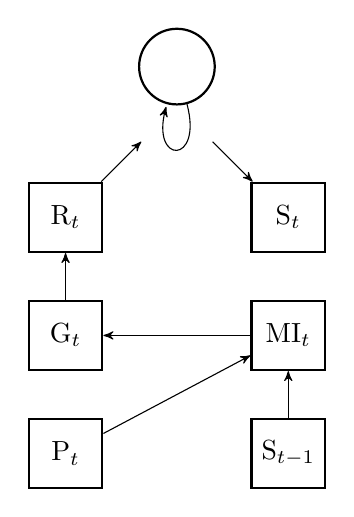
\begin{tikzpicture}[->,>=stealth',auto,thin]
\tikzstyle{every state}=[shape=rectangle,draw,thick,text=black, text centered, text width=0.7cm, align=center]

\node[state]		(A) [shape=circle]             {};
\node[state]        (B) [below of=A, node distance=0.5cm,draw=none] {};
\node[state]		(C) [below left of=B,node distance=2cm] {R$_{t}$};
\node[state]		(D) [below of=C,node distance=1.5cm] {G$_{t}$};
\node[state]        (E) [below of=D,node distance=1.5cm] {P$_{t}$};
\node[state]		(F) [below right of=B,node distance=2cm] {S$_{t}$};
\node[state]		(G) [below of=F,node distance=1.5cm] {MI$_{t}$};
\node[state]		(H) [below of=G,node distance=1.5cm] {S$_{t-1}$};


\path
(A) edge[loop below] (A)
(B) edge (F)
(C) edge (B)
(D) edge (C)
(E) edge (G)
(G) edge (D)
(H) edge (G);
\end{tikzpicture}
\caption{}
\label{fig:subfig2}
\end{subfigure}
\begin{subfigure}[b]{0.3\textwidth}
    \centering
    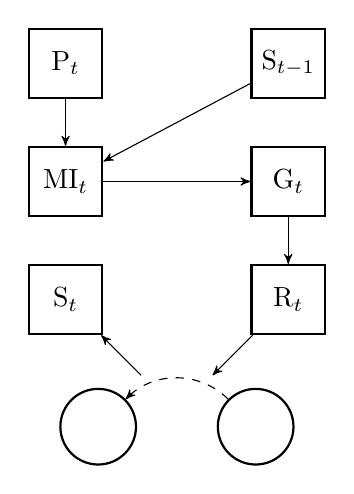
\begin{tikzpicture}[->,>=stealth',auto,thin]
\tikzstyle{every state}=[shape=rectangle,draw,thick,text=black, text centered, text width=0.7cm, align=center]

\node[state]		(A) [shape=circle]             {};
\node[state]        (B) [right of=A, node distance=2cm,shape=circle] {};
\node[state]        (C) [right of=A, node distance=1cm,draw=none] {};
\node[state]        (D) [above of=C, node distance=0.2cm,draw=none] {};
\node[state]		(E) [above left of=D,node distance=2cm] {S$_{t}$};
\node[state]		(F) [above of=E,node distance=1.5cm] {MI$_{t}$};
\node[state]		(G) [above of=F,node distance=1.5cm] {P$_{t}$};
\node[state]        (H) [above right of=D,node distance=2cm] {R$_{t}$};
\node[state]		(I) [above of=H,node distance=1.5cm] {G$_{t}$};
\node[state]		(J) [above of=I,node distance=1.5cm] {S$_{t-1}$};
\path
(B) edge[dashed,bend left=-45] (A)
(D) edge (E)
(F) edge (I)
(G) edge (F)
(H) edge (D)
(I) edge (H)
(J) edge (F)
;
\end{tikzpicture}
\caption{}
\label{fig:subfig3}
\end{subfigure}
\begin{subfigure}[b]{0.3\textwidth}
    \centering
    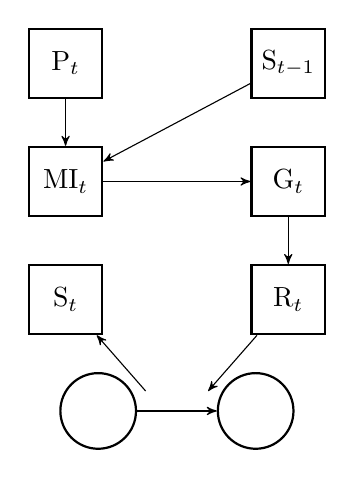
\begin{tikzpicture}[->,>=stealth',auto,thin]
\tikzstyle{every state}=[shape=rectangle,draw,thick,text=black, text centered, text width=0.7cm, align=center]

\node[state]		(A) [shape=circle]             {};
\node[state]        (B) [right of=A, node distance=2cm,shape=circle] {};
\node[state]        (C) [right of=A, node distance=1cm,draw=none] {};
\node[state]        (D) [below of=C, node distance=0.2cm,draw=none] {};
\node[state]		(E) [above left of=C,node distance=2cm] {S$_{t}$};
\node[state]		(F) [above of=E,node distance=1.5cm] {MI$_{t}$};
\node[state]		(G) [above of=F,node distance=1.5cm] {P$_{t}$};
\node[state]        (H) [above right of=C,node distance=2cm] {R$_{t}$};
\node[state]		(I) [above of=H,node distance=1.5cm] {G$_{t}$};
\node[state]		(J) [above of=I,node distance=1.5cm] {S$_{t-1}$};

\path
(A) edge (B)
(D) edge (E)
(F) edge (I)
(G) edge (F)
(H) edge (D)
(I) edge (H)
(J) edge (F)
;
\end{tikzpicture}
\caption{}
\label{fig:subfig4}
\end{subfigure}

\caption{Graphical representation of the female human life cycle (a) and the influence of resource dynamics in survival (b) and reproductive (c) dynamics. The female human life cycle (a) is represented with a life cycle graph, dividing the life cycle in four stages: J as the sexually immature stage (i.e. juvenile), A as the sexually mature but without descendants stage (i.e. adult), RC as the stage where individuals reproduce (i.e. reproductive career), and PR as the stage where individuals no longer can reproduce (i.e. post-reproductive). The influence of resource dynamics in survival (b), reproduction (c) and life cycle stage transition (d), is based on the amount of resources stored from the last iteration (S$_{t-1}$), the amount of resources produced (P$_{t}$), received (R$_{t}$), and gave away (G$_{t}$) in the current iteration, as well as the maternal investment (MI$_{t}$). The resources stored from one iteration to the next one (S$_{t}$) are the amount left after the resource dynamics and the life cycle dynamics of survival, reproduction, and transition. Loop arrows below life cycle stages refers to the probability of staying in that stage (i.e. survival). A newborn is produced either when an individual transition from stage A to RC or when an individual remains in stage RC. The dashed arrows refers to the production of a descendant in that life cycle (i.e. reproduction). The dashed arrow from A to J refers to the age at first reproduction, which is also the transition from A to RC, whereas the one from RC to J refers to reproduction within the reproductive career. The thick arrows between life cycle stages refers to the transition from one stage to the other. The thick arrows between resource dynamics refers to the relationship among them, and which one is used to evaluate survival, reproduction, and life cycle stage transition}.
    \label{fig:1}
\end{figure}

\clearpage

\begin{algorithm}[H]
    \caption{Simulation of a Population}
    \begin{algorithmic}
    \State Generate initial data frame of $N$ random adults
    \State Define stage-specific maximum resource production ($\beta$)
    \State Define stage-specific production probabilities ($\gamma$)
    \State Define block matrix ($\delta$)
    \State Define survival threshold ($\epsilon$)
    \State Define reproductive threshold ($\eta$)
        \For {iteration=1,2, \ldots, $T$}
        \State Compute the amount of resources produced
        \State $prod = rbinom(1,\beta_{stage},\gamma_{stage})$
        \State Update stored resources
        
        \If{$store_{mother} > \epsilon$ and $store_{desc} < \epsilon$}
        \State Compute need-based maternal investment
        \State Update stored resources
        \EndIf
        
        \If{$store > \epsilon$}
        \State Compute maximum out degree
        \State Generate social network
        \State Record out degree and in degree
        \State Update stored resources
        \EndIf
        
        \If{$store \geq \epsilon + \eta$}
        \State Reproduce and discount reproductive threshold
        \State Update stored resources
        \Else
        \State Do not reproduce
        \EndIf
        
        \If{juvenile and older than 10 yo and $store \geq \epsilon + \eta$ OR juvenile and older than 18 yo}
        \State Transition to adult stage and discount reproductive threshold
        \ElsIf{adult and $store \geq \eta$}
        \State Go through reproductive dynamics and transition to reproductive career stage
        \ElsIf{reproductive career and older than 40 yo and have not reproduced in the last 10 years and $store \leq + \eta$ OR older than 60 yo}
        \State Transition to post-reproductive stage
        \EndIf
        
        \If{$store \geq \epsilon$}
        \State Survive and age
        \State Update stored resources
        \Else
        \State Die
        \EndIf
        
        \State Update population

        \EndFor
        \State $store = prod - mat_{inv} - out_{deg} + in_{deg} - \eta - \epsilon$

    \end{algorithmic} 
    \label{alg:people}
\end{algorithm} 

\clearpage

\bibliographystyle{apalike}
\bibliography{optimal_ref}

\end{document}
